% !TeX spellcheck = en-US
% !TeX encoding = utf8
% !TeX program = lualatex
% !BIB program = biber
% -*- coding:utf-8 mod:LaTeX -*-


% vv  scroll down to line 200 for content  vv


\let\ifdeutsch\iffalse
\let\ifenglisch\iftrue
\input{pre-documentclass}
\documentclass[
  % fontsize=11pt is the standard
  a4paper,  % Standard format - only KOMAScript uses paper=a4 - https://tex.stackexchange.com/a/61044/9075
  twoside,  % we are optimizing for both screen and two-side printing. So the page numbers will jump, but the content is configured to stay in the middle (by using the geometry package)
  bibliography=totoc,
  %               idxtotoc,   %Index ins Inhaltsverzeichnis
  %               liststotoc, %List of X ins Inhaltsverzeichnis, mit liststotocnumbered werden die Abbildungsverzeichnisse nummeriert
  headsepline,
  cleardoublepage=empty,
  parskip=half,
  %               draft    % um zu sehen, wo noch nachgebessert werden muss - wichtig, da Bindungskorrektur mit drin
  draft=false
]{scrbook}
\input{config}


\usepackage[
  title={Analysis and Transfer of AutoML Concepts for Clustering Algorithms},
  author={Dennis Tschechlov},
  type={Master Thesis},
  institute=ipvs, % or other institute names - or just a plain string using {Demo\\Demo...}
  course={Softwaretechnik},
  examiner={PD Dr. rer. nat. habil. Holger Schwarz},
  supervisor={Manuel Fritz,\ M.Sc.},
  startdate={June 20, 2019},
  enddate={December 20, 2019}
]{scientific-thesis-cover}

\usepackage{booktabs}
\usepackage{graphicx}

\usepackage{ amssymb }
\newcommand{\Lcurv}{\mathcal{L}}
\DeclareMathOperator*{\argmin}{\arg\!\min}
% Hier stehen alle Abkürzungen
\newacronym{er}{ER}{error rate}
\newacronym{fr}{FR}{Fehlerrate}
\newacronym[plural={RDBMS},shortplural={RDBMS}]{rdbms}{RDBMS}{Relational Database Management System}
\newacronym{SH}{SH}{SuccessiveHalving}
\newacronym{AutoML}{AutoML}{Automated machine learning}
\newacronym{NAS}{NAS}{Neural architecture search}
\newacronym{BOHB}{BOHB}{Bayesian Optimization and Hyperband}
\newacronym{EI}{EI}{expected improvement}
\newacronym{BHO}{BHO}{Bayesian Hyperparameter Optimization}
\newacronym{SMAC}{SMAC}{Sequential model-based algorithm configuration}
\newacronym{CASH}{CASH}{Combined Algorithm and Hyperparameter Optimization}
\newacronym{SMAC}{SMAC}{Sequential Model-based Algorithm Con- figuratio}
\newacronym{TPE}{TPE}{Tree-structured Parzen Estimator}


\makeindex

\begin{document}

%tex4ht-Konvertierung verschönern
\iftex4ht
  % tell tex4ht to create picures also for formulas starting with '$'
  % WARNING: a tex4ht run now takes forever!
  \Configure{$}{\PicMath}{\EndPicMath}{}
  %$ % <- syntax highlighting fix for emacs
  \Css{body {text-align:justify;}}

  %conversion of .pdf to .png
  \Configure{graphics*}
  {pdf}
  {\Needs{"convert \csname Gin@base\endcsname.pdf
      \csname Gin@base\endcsname.png"}%
    \Picture[pict]{\csname Gin@base\endcsname.png}%
  }
\fi

%\VerbatimFootnotes %verbatim text in Fußnoten erlauben. Geht normalerweise nicht.

\input{commands}
\pagenumbering{arabic}
\Titelblatt

%Eigener Seitenstil fuer die Kurzfassung und das Inhaltsverzeichnis
\deftripstyle{preamble}{}{}{}{}{}{\pagemark}
%Doku zu deftripstyle: scrguide.pdf
\pagestyle{preamble}
\renewcommand*{\chapterpagestyle}{preamble}



%Kurzfassung / abstract
%auch im Stil vom Inhaltsverzeichnis
\ifdeutsch
  \section*{Kurzfassung}
\else
  \section*{Abstract}
\fi

<Short summary of the thesis>

\cleardoublepage


% BEGIN: Verzeichnisse

\iftex4ht
\else
  \microtypesetup{protrusion=false}
\fi

%%%
% Literaturverzeichnis ins TOC mit aufnehmen, aber nur wenn nichts anderes mehr hilft!
% \addcontentsline{toc}{chapter}{Literaturverzeichnis}
%
% oder zB
%\addcontentsline{toc}{section}{Abkürzungsverzeichnis}
%
%%%

%Produce table of contents
%
%In case you have trouble with headings reaching into the page numbers, enable the following three lines.
%Hint by http://golatex.de/inhaltsverzeichnis-schreibt-ueber-rand-t3106.html
%
%\makeatletter
%\renewcommand{\@pnumwidth}{2em}
%\makeatother
%
\tableofcontents

% Bei einem ungünstigen Seitenumbruch im Inhaltsverzeichnis, kann dieser mit
% \addtocontents{toc}{\protect\newpage}
% an der passenden Stelle im Fließtext erzwungen werden.

\listoffigures
\listoftables

%Wird nur bei Verwendung von der lstlisting-Umgebung mit dem "caption"-Parameter benoetigt
%\lstlistoflistings 
%ansonsten:
\ifdeutsch
  \listof{Listing}{Verzeichnis der Listings}
\else
  \listof{Listing}{List of Listings}
\fi

%mittels \newfloat wurde die Algorithmus-Gleitumgebung definiert.
%Mit folgendem Befehl werden alle floats dieses Typs ausgegeben
\ifdeutsch
  \listof{Algorithmus}{Verzeichnis der Algorithmen}
\else
  \listof{Algorithmus}{List of Algorithms}
\fi
%\listofalgorithms %Ist nur für Algorithmen, die mittels \begin{algorithm} umschlossen werden, nötig

% Abkürzungsverzeichnis
\printnoidxglossaries

\iftex4ht
\else
  %Optischen Randausgleich und Grauwertkorrektur wieder aktivieren
  \microtypesetup{protrusion=true}
\fi

% END: Verzeichnisse


% Headline and footline
\renewcommand*{\chapterpagestyle}{scrplain}
\pagestyle{scrheadings}
\pagestyle{scrheadings}
\ihead[]{}
\chead[]{}
\ohead[]{\headmark}
\cfoot[]{}
\ofoot[\usekomafont{pagenumber}\thepage]{\usekomafont{pagenumber}\thepage}
\ifoot[]{}


%% vv  scroll down for content  vv %%































%%%%%%%%%%%%%%%%%%%%%%%%%%%%%%%%%%%%%%%%%%%%%%%%%%%%%%%%%%%%%%%%%%%%%%%%%%%%%%
%
% Main content starts here
%
%%%%%%%%%%%%%%%%%%%%%%%%%%%%%%%%%%%%%%%%%%%%%%%%%%%%%%%%%%%%%%%%%%%%%%%%%%%%%%


\chapter{Introduction}
\label{chap:intro}
\begin{itemize}
    \item A lot of data today ...
    \item Data analysis is an highly exploratory task
    \item Many processes to do the analysis, one example is the Knowledge Discovery in Databases (KDD) process (see \cref{fig:kdd}).
    \begin{figure}
        \centering
        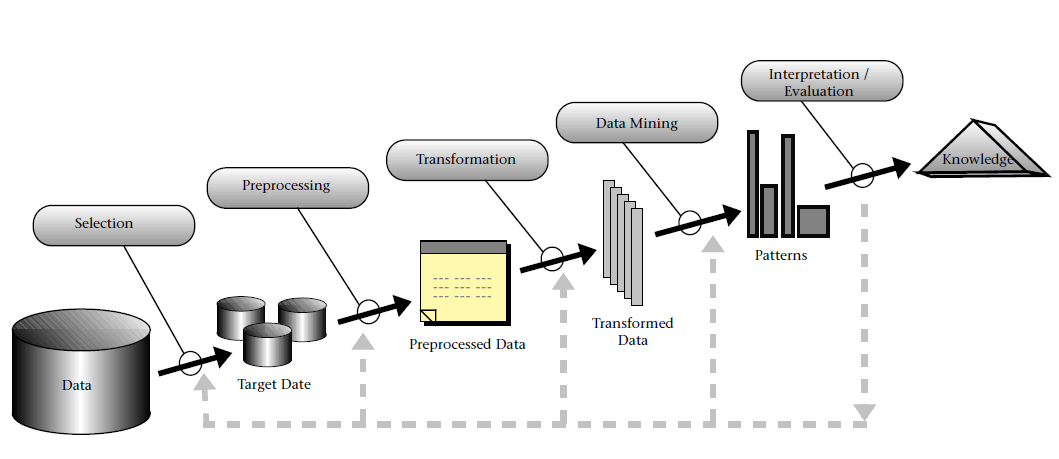
\includegraphics[width=\textwidth]{graphics/kdd_process.png}
        \caption{Overview of the KDD process \cite{Fayyad:1996:DMK:257938.257942}.}
        \label{fig:kdd}
    \end{figure}
    \item All process in common that iterative steps
    \item Focus of this work is in the data mining and evaluation step
    \item There are different steps involved here
    \item Important ones are the algorithm selection, the hyperparameter selection and the evaluation
    \item Human experts contribute to this steps by using their domain knowledge and experiences.
    \item Adjust parameters and algorithms. This is a trial-and-error process which takes a lot of time.
    \item  Also not always clear how to adjust parameters and algorithms.
    \item There are a lot of research in this area to help the analyst.
    One are so called \textit{White-box} methods.
    These methods aim at increasing the traceability by explaining the results of machine learning models to the analyst.
    Nevertheless, the choice of choosing an appropriate algorithm and its hyperparameters lies with the analyst.
    \item The other methods are \textit{Black-box} methods.
    In contrast to White-box methods, Black-box methods try to optimize machine learning models by automatically selecting an appropriate algorithm and its hyperparameters.
    But as the name suggest it is not clear what is happening inside this methods.
    The benefit of this methods is that they can be used without any expert knowledge and that they can lead to  higher accuracy and runtime savings compared to White-box methods.
    \item White-box = Human-in-the-loop
    \item Black-box = Take Human-out-of-the-loop
    \item Additionally, Black-box methods can be used without expert knowledge and still are able to achieve promising results.
    \item This research field is also known as \gls{AutoML}.
    Currently, there are a lot of \gls{AutoML} systems \todo{cite here the automl systems}.
    The general idea of this systems is shown in \cref{fig:automlWorkflow}.
    \begin{figure}
        \centering
        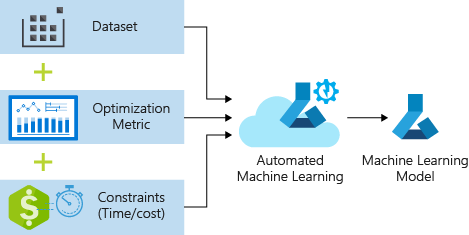
\includegraphics[width=0.5\textwidth]{graphics/flow_autom.png}
        \caption{Basic overview of the functionality of AutoML systems.}
        \label{fig:automlWorkflow}
    \end{figure}
    The inputs for the systems are three things: 
    \begin{itemize}
        \item The input datasets which have to be analyzed.
        \item A metric, according to which  the best model is searched.
        \item A constraint or budget, which can be for example a time budget of one hour.
        This means that the AutoML system terminates after one hour and returns the best model that was found in this time budget.
    \end{itemize}
    The input datasets, a metric, according to which the optimal model is searched and a constraint which  
    
    \item Some of this systems also learn from the performance of algorithms that were used in the past and transfer this knowledge to new unseen datasets, which is known as \textit{Meta-learning}.
    \item These systems do only cover supervised learning algorithms like classification.
    But many problems in Data Mining do not have the class label information.
    Hence, only unsupervised learning algorithms can be applied to this problems.
    Because of the missing class labels the concepts of the existing \gls{AutoML} systems cannot be applied directly.
    Therefore, for unsupervised learning there are only some approaches to use meta-learning but they all do not cover the combined problem of algorithm selection and hyperparameter optimization, which is known as \gls{CASH} problem.
    Also, they do not use the optimization methods to tune the hyperparameters that were used in the existing AutoML systems.
    \item Due to the limited work in this area, the goal of this work is to transfer these concepts of optimization methods and meta-learning on the unsupervised learning task clustering to solve the \gls{CASH} problem.
\end{itemize}
 The remainder of this paper is structured as follows ...
\xtodo{add this}



\chapter{Background}
\label{chap:background}

In this chapter the needed background for this work will be shown.
Therefore, first the AutoML concept in general will be explained.
Then the optimization techniques that are used in AutoML systems will be shown.
These optimization techniques require metrics as input.
So, the metrics that are available for clustering will be presented.
Afterwards the concept of Meta-learning will be described.

\section{AutoML}
The problem of \gls{AutoML} is to produce automatically, so without human input, test set predictions for a given test set within a resource budget $b$.
This can be formally defined as shown in \Cref{def:automl}.

\begin{definition}[\gls{AutoML} problem]
\label{def:automl}
For $i = 1, \dots, n+m$ let $x_i \in \mathbb{R}^d$ denote a feature vector and $y_i \in Y $ the corresponding target value.
Given training data $D_{train} = \lbrace (x_1, y_1), \dots, (x_n, y_n) \rbrace $ and the feature vectors $x_{n+1, \dots, n+m}$ of a test dataset $D_{test} = \lbrace (x_{n+1}, y_{n+1}), \dots, (x_{n+m}, y_{n+m})  \rbrace$ drawn from same underlying distribution, as well as a ressource budget $b$ and a loss metric $\mathbb{L}(\cdot, \cdot)$, the \gls{AutoML} problem is to automatically produce test set predictions $\hat{y}_{n+1}, \dots, \hat{y}_{n+m}$ such that the loss 
\begin{equation*}
    \frac{1}{m} \sum_{j=1}^m \Lcurv(\hat{y}_j, y_j)
\end{equation*}
is minimized.
\end{definition}


Many \gls{AutoML} systems do not directly address the problem described in \Cref{def:automl}, but they see the \gls{AutoML} problem as \gls{CASH} problem \cite{Feurer2015EfficientLearning,  Kotthoff2017Auto-WEKAWEKA}. 
This is because the main problems of \gls{AutoML} are that first there is no single algorithm that performs best on every dataset and the choice of hyperparameter is crucial for the performance of an algorithm.
The \gls{CASH} problem is formally defined in \Cref{def:cash}.

\begin{definition} [\gls{CASH} problem]
\label{def:cash}
Let $A^(1), \dots, A^(R)$ be a set of algorithms, where the hyperparameters of each algorithm have the domain $\Lambda^(i)$.
Alos, let $ D_{train} =  \lbrace (x_1, y_1), \dots, (x_n, y_n) \rbrace$ be a training set which is split into k  disjunct cross-validation folds $\lbrace D^{(1)}_{valid}, \dots, D^{(k)}_{valid} \rbrace$ and $\lbrace D^{(1)}_{train}, \cdots, D^{(k)}_{train} \rbrace$  such that $D^{(i)}_{train} = D_{train} \textbackslash D^{(i)}_{valid}$ for $i=1, \dots, k$.
Finally, let $L( A^{(i)}_{\lambda}, D^{(i)}_{train}, D^{(i)}_{valid})$ denote the loss that algorithm $A^{(i)}$ has on $D^{(i)}_{valid}$ when trained on $D^{(j)_{train}}$ with hyperparameters $\lambda$.
Then, the \gls{CASH} problem is to find the joint algorithm and hyperparameter setting that minimizes the loss:
\begin{equation*}
    A^*, \lambda^* \in \underset{A^{(j)}\in A, \lambda \in \Lambda^{(j)}}{argmin} \frac{1}{k} \sum_{i=1}^k \Lcurv(A^{(j)}_{\lambda}, D^{(i)}_{train}, D^{(i)}_{valid})
\end{equation*}

\end{definition}



\section{Hyperparameter Optimization Techniques for Classification}

\begin{itemize}
    \item Hyperparameter optimization in general, describe the problem of finding parameter configuration that maximizes the validation performance.
    \item 
\end{itemize}
In this section methods for the optimization of hyperparameters that are used in AutoML systems will be described.

Most of the methods have three steps in common, which are:
\begin{enumerate}
    \item Run the current model.
    \item Evaluate the results of the current model according to a metric.
    \item Select the next model that should be run.
\end{enumerate}
The difference in the methods is how they select the next model that will be run, so step 3 above. 

The methods that will be presented are shown in \cref{fig:hpo} and can generally be divided into three categories \cite{Li2017Hyperband:Optimization,BergstraAlgorithmsOptimization, Falkner2018BOHB:Scale, Feurer2015EfficientLearning}:
\begin{figure}
    \centering
    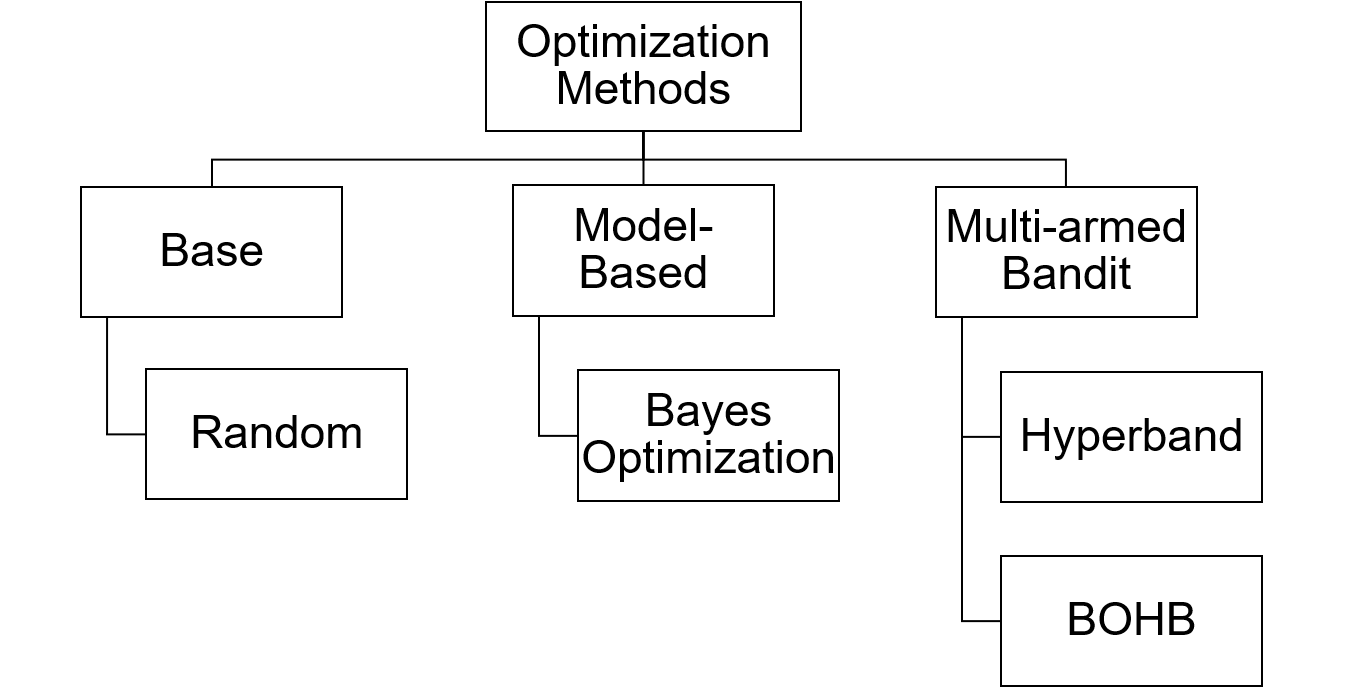
\includegraphics[width=0.5\textwidth]{data/HPO_methods.png}
    \caption{Overview of the hyperparameter optimization methods that will be described.}
    \label{fig:hpo}
\end{figure}
\begin{itemize}
    \item \textbf{Base}: Methods that are basically used like Random-search.
    Like the name suggests, Random-search is running random configurations and evaluates them.
    \item \textbf{Sequential model-based}: Methods that create a model of the hyperparameters to predict the best hyperparameters.
    One representative of this class is the \gls{BHO}
    \item \textbf{Multi-armed Bandit}: These methods try to sample a lot of configurations in parallel with a very low budget for each configuration.
    Examples for this class are Hyperband and \gls{BOHB}, which is a combination of \gls{BHO} and Hyperband.
\end{itemize}

In the following these methods will be described in more detail.
Of course, there are also other methods like gradient-based methods, but in the following only those methods will be presented that have proven to work well in the AutoML systems.


\subsection{Random}

\begin{itemize}
    \item One of the most simple Hyperparameter optimization methods is Random \cite{Bergstra:2012:RSH:2503308.2188395}.
    \item Though can be very effective, especially if the search space is not very large.
    \item Performs in general better than Gridsearch.
    \item Fails for large and high-dimensional parameter spaces.
    
\end{itemize}

\subsection{Bayes Optimization}

\begin{itemize}
    \item Model-based method that relies on a statistical model and an acquisition function \cite{ShahriariTakingOptimization, Frazier2018AOptimization, SnoekPracticalAlgorithms}.
    Goal of acquisition function is to find a sample that should be evaluated next.
    Should make trade-off between exploration and exploitation.
    \item Only a framework, several implementations with different models and acquisition functions.
    \item Surrogate model about how the objective function (parameter configuration to metric value).
    \item An example for an often used statistical model are Gaussian Processes (GP) \cite{ShahriariTakingOptimization}.
    \item Goal is to approximate this model by samples.
    \item The steps are:
    \begin{itemize}
        \item select next parameter configuration that maximizes the acquisition function.
        \item Run model with these parameter configuration.
        \item Evaluate the configuration, so calculate metric(configuration).
        \item Update the model.
    \end{itemize}
    \item An example for this procedure is shown in \cref{fig:BOExample}. 
    
    \begin{figure}
        \centering
        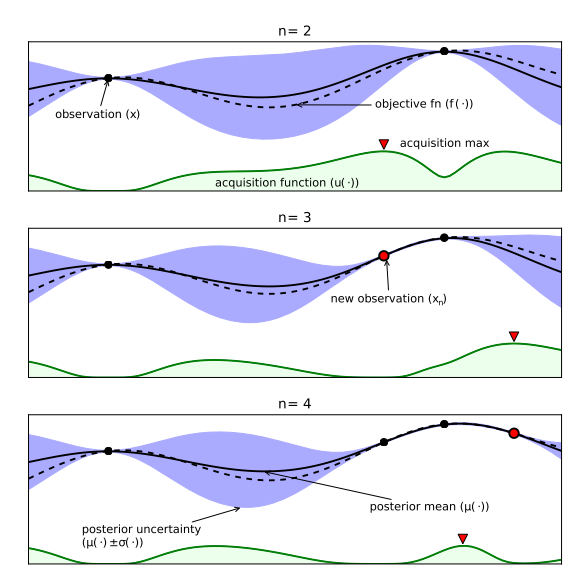
\includegraphics{graphics/bayes_optimization_example.png}
        \caption{Example of the Bayesian Optimization procedure \cite{ShahriariTakingOptimization}.}
        \label{fig:BOExample}
    \end{figure}
    \item Example for an acquisition function is the \gls{EI}:
    \begin{equation}
        a(x) = \int max(0, \alpha -f(x)) dp(f|D)
    \end{equation}
    Here $\alpha$ is the currently best observed value.
    \item One implementation of the Bayes optimization is the Tree Parzen Estimator (TPE) \cite{BergstraAlgorithmsOptimization}, which uses a density kernel estimator.
    
    \item Should only be used if f has no closed form or is expensive to evaluate.
    \item Sequential, so no parallelization.
    \item Only good after some samples, for less samples random could be better.
\end{itemize}

\subsection{Hyperband}

Hyperband \cite{Li2017Hyperband:Optimization} is a multi-armed bandit method that relies on \gls{SH} \cite{Jamieson2015Non-stochasticOptimization}.
The general algorithm is shown in \cref{fig:HBAlgorithm}.
\begin{figure}
    \centering
    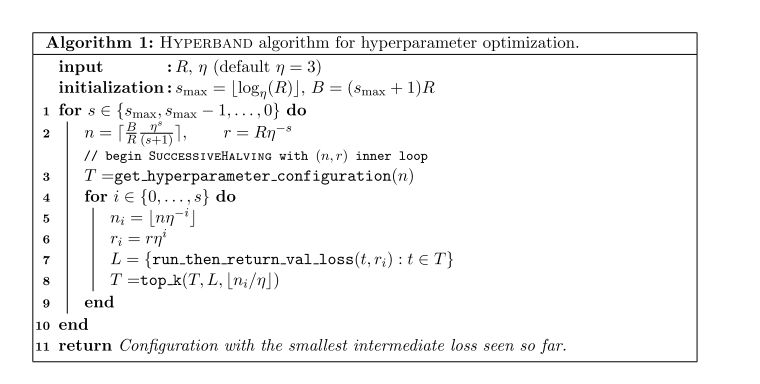
\includegraphics[width=\textwidth]{graphics/hyperband_algorithm.png}
    \caption{Overview of the Hyperband algorithm \cite{Li2017Hyperband:Optimization}.}
    \label{fig:HBAlgorithm}
\end{figure}

\begin{itemize}
    \item Gets as input the maximum budget for one configuration and $\eta$, which controls the amount of configurations that are discarded after each round of \gls{SH}.
    \item The general idea is to run many \gls{SH} runs.
    \item One SH run consists of many iterations. First random configurations are sampled.
    The number of configurations should be chosen in such a way that the minimum budget can be distributed equally over all configurations.
\end{itemize}

\subsection{Bayesian Optimization and Hyperband}

\gls{BOHB} is a combination of the Bayesian Optimization and the Hyperband method.
Instead of random sampling of configurations in the different \gls{SH} iterations of Hyperband, \gls{BOHB} uses Bayesian Optimization to fit a model and to select the configurations.
 

\section{Clustering Algorithms}

\begin{itemize}
    \item What is clustering
    \item what is partitional clustering
    \item which partitional clustering algorithms exist
    \item shortly explain the algorithms that are used in the implementation (GMM, KMeans, KMedoids)
\end{itemize}

\section{Clustering Metrics}
\begin{itemize}

    \item Metric Types: internal, external, relative (?)
    \item explain how they work and use show metrics that are used in the concept/implementation.
\end{itemize}

\section{Meta-learning}

Meta-learning \cite{Brazdil2010MetalearningMining.} is the task of learning to learn.
In the area of machine learning it can be used to learn algorithms and their configurations from previous tasks.
For this, it typically includes an offline and an online phase.
The basic workflow is shown in \cref{fig:metalearningArch}.
\begin{figure}
    \centering
    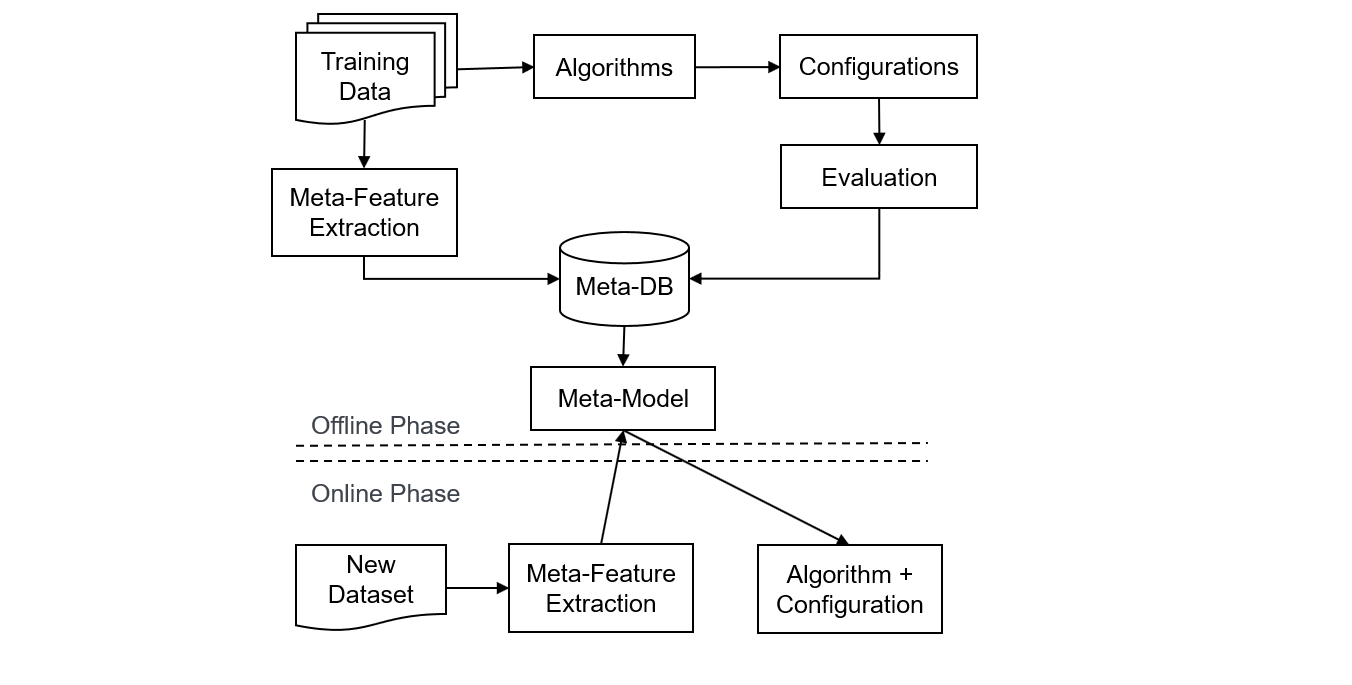
\includegraphics[width=\textwidth]{graphics/metalearning_general_architecture.png}
    \caption{General architecture of meta-learning, divided into offline and online phase.}
    \label{fig:metalearningArch}
\end{figure}

\begin{itemize}
    \item In an offline phase, training data is needed (which represents previous tasks).
    \item From this training data, \textit{meta-features} are extracted.
    Describe characteristics of the dataset.
    Example can be number of instances or number of attributes.
    \item meta-features of a dataset are saved in a database (meta-db in the figure).
    \item Then for the dataset, different algorithms with different configurations are run and evaluated.
    The configurations as well as the result of the evaluations are also stored in the meta-db.
    From meta-db information meta-learner can be derived.
    \item Online Phase: If new dataset, then first have to extract meta-features.
    \item Meta-features are input for meta-learner.
    \item Meta-learner suggests promising algorithm with configuration based on the meta-db knowledge.
    \item One possibility is to find the most similar dataset according to meta-features and then take best known algorithm and configuration from meta-db.
    \item This would correspond to a k-Nearest-Neighbor classifier with $k=1$.
    \item Question is which meta-features should be used.
    \item Meta-features can be categorized into five groups \cite{Rivolli2018TowardsMeta-learning}:
    \begin{itemize}
        \item \textbf{Simple}: Can be directly extracted from the data and include measure like the number of instances or the number of attributes.
        \item \textbf{Statistical}: Measure statistical information about the data.
        They include measure like mean, median, standard deviation etc.
        \item \textbf{Information-theoretic}: Based on entropy and capture the information and the complexity in the data.
        An example is the attribute entropy.
        \item \textbf{Model-based}: This group of meta-features use structural properties of machine learning models.
        For example they build a decision tree from the data and the number of leaves of that tree is one meta-feature.
        \item \textbf{Landmarking}: The landmarking meta-features use the performance of simple classifiers like Naive Bayes as meta-features.
    \end{itemize}
    
    \item Landmarking and model-based cannot be used for clustering since we are assuming in the online phase of meta-learning that there are no class labels. 
    \item Other groups also contain meta-features with class labels, e.g., the number of classes. For this work only those without class labels are interesting.
\end{itemize}

\chapter{Related Work}
\label{chap:related}
In this section the related work will be presented.
For this, the related work is categorized into three categories:
\begin{itemize}
    \item \gls{AutoML} frameworks for classification
    \item Parameter optimization for clustering. 
    \item Meta learning for clustering
\end{itemize}

The related work for these categories will be shown in the following sections.

\section{AutoML Frameworks for classification}

In this section, two AutoML systems will be described in more detail.
These are Auto-Weka and Auto-sklearn.

\subsection{Auto-Weka}
\begin{itemize}
    \item Auto-Weka \cite{ThorntonAuto-WEKA:Algorithms, Kotthoff2017Auto-WEKAWEKA} was one of the first \gls{AutoML} systems.
    \item Used Bayesian Optimization to tackle the \gls{CASH} problem.
    \item Actually, \gls{BO} only for hyperparameter selection, but they used the algorithm as top-level parameter and depending on that value they selected the other hyperparameters.
    \item Basic architecture is shown in \cref{fig:autoweka}.
    Input for the system is budget, training data and a metric, according to which the optimizer is going to find the best model.
    As long as budget is left, the optimizer runs, which means the model is executed on the training data, then evaluated, stored and then the most important part, the next model is selected.
    \item Model has to be chosen in intelligent way, because limited budget and not able to search whole algorithm and their hyperparameter space.
    \item Optimizer there is Bayes Optimizer, more specifically they used \gls{SMAC} \cite{HutterSequentialConfiguration} and \gls{TPE} \cite{BergstraAlgorithmsOptimization}.
    \begin{figure}
        \centering
        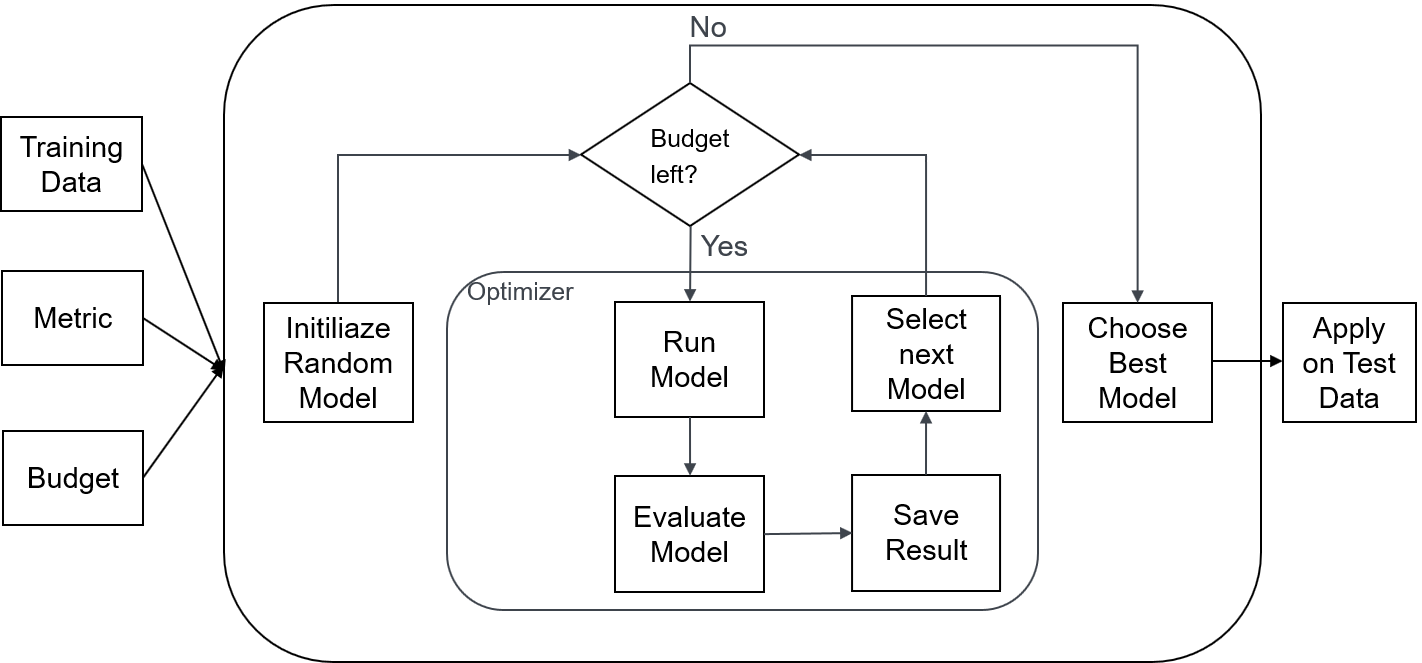
\includegraphics[width=0.7\textwidth]{graphics/auto_weka_arch.png}
        \caption{General architecture of the Auto-Weka system.}
        \label{fig:autoweka}
    \end{figure}
    \item Took all classifiers available in Auto-Weka. 
    They also used two ensemble classifiers and treated them as classifiers, but they only allowed five classifiers at maximum in the ensemble, such that the configuration space does not get too large.
    \item They were able to show that this approach is better than just running all algorithms with default hyperparameters and then choosing the best one (according to metric).
    \item They also showed that there approach performs in 11/21 cases with \gls{SMAC} and in 4/21 cases with \gls{TPE} regarding the test performance. Random Search in 2/21 and Grid Search in 4/21 cases.
\end{itemize}

\subsection{Auto-sklearn}
Auto-sklearn \cite{Feurer2015EfficientLearning} is based on the machine learning library scikit-learn \cite{PedregosaFABIANPEDREGOSA2011Scikit-learn:Perrot}.
They built the concept based on the Auto-Weka concept and extended it with two components.
\begin{itemize}
    \item General architecture of Auto-sklearn is shown in \cref{fig:autosklearn}.
    \begin{figure}
        \centering
        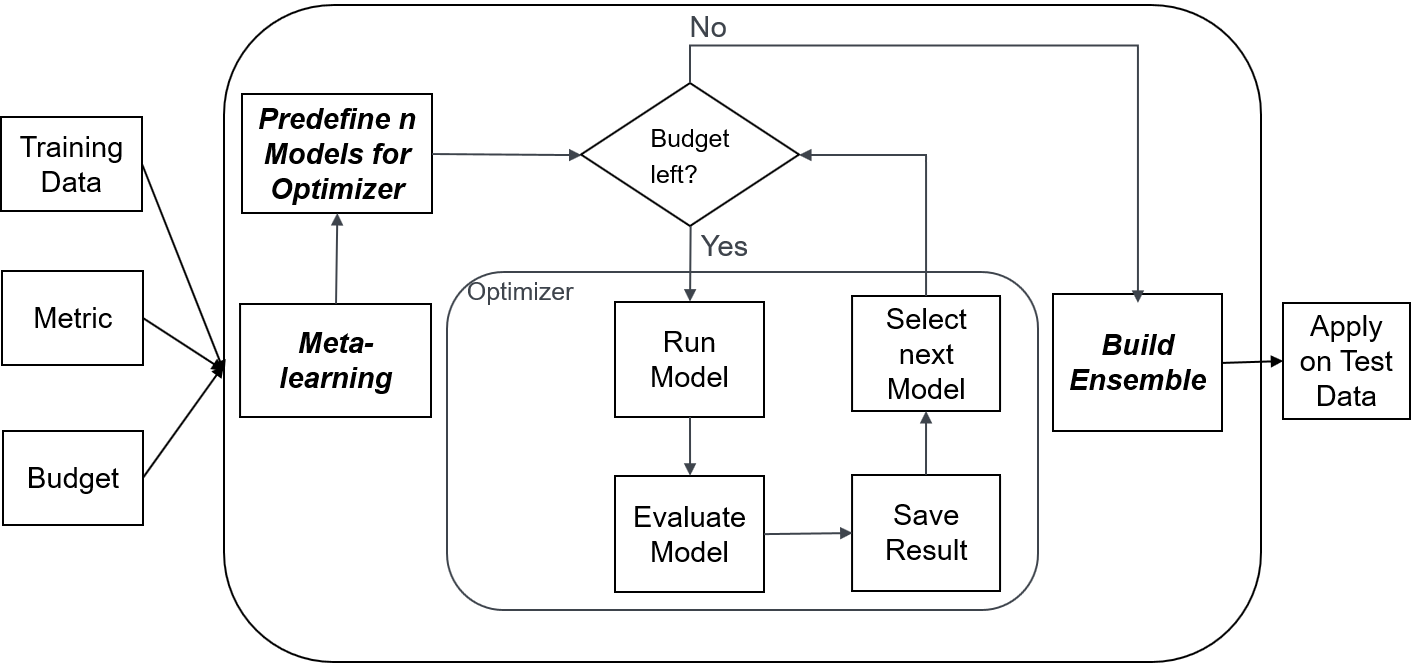
\includegraphics[width=0.7\textwidth]{graphics/auto_sklearn_arch.png}
        \caption{Basic architecture of Auto-sklearn. The components that are added compared to the Auto-Weka system (see \cref{fig:autoweka}) are marked as bold.}
        \label{fig:autosklearn}
    \end{figure}
    \item General same as Auto-Weka but \textit{meta-learning} and \textit{build ensemble} components are added.
    \item 
\end{itemize}

\iffalse

The basic architecture of their approach is shown in \Cref{fig:autosklearnArch}.
\begin{figure}
\centering
    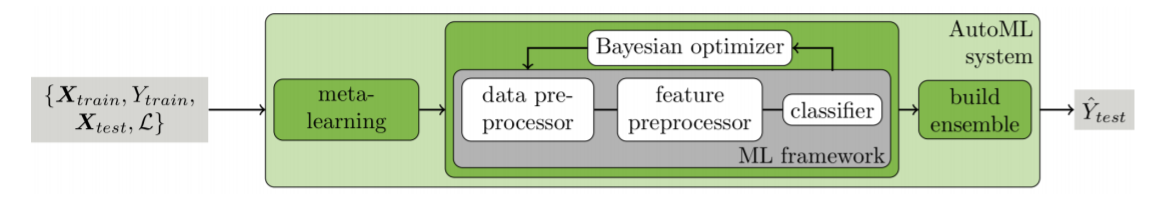
\includegraphics[width=\textwidth]{graphics/autosklearn_architecture.png}
    \caption{Basic workflow of the AUTO-SKLEARN system \cite{Feurer2015EfficientLearning}.}
    \label{fig:autosklearnArch}
\end{figure}
\fi

Meta-learning \cite{Brazdil2010MetalearningMining.} is a  method that learns from the performance of learning algorithms across datasets and applies it on new unseen datasets.
For this 38 meta-features, which represent the characteristics of a dataset, were extracted from the training datasets in an offline phase.
They also run SMAC \cite{HutterSequentialConfiguration} for 24 hours with 10-fold cross-validation on two-thirds of the data and the ML instance that had the best performance on the third one was stored.
In the online phase, for a new dataset, the meta-features were extracted and the datasets from the offline phase were ranked by the $L_1$ distance. 
The ML algorithms (that performed best in offline phase) of the 25 nearest datasets were then used and Bayesian optimization were run on them.
\iffalse
\begin{figure}
\centering
    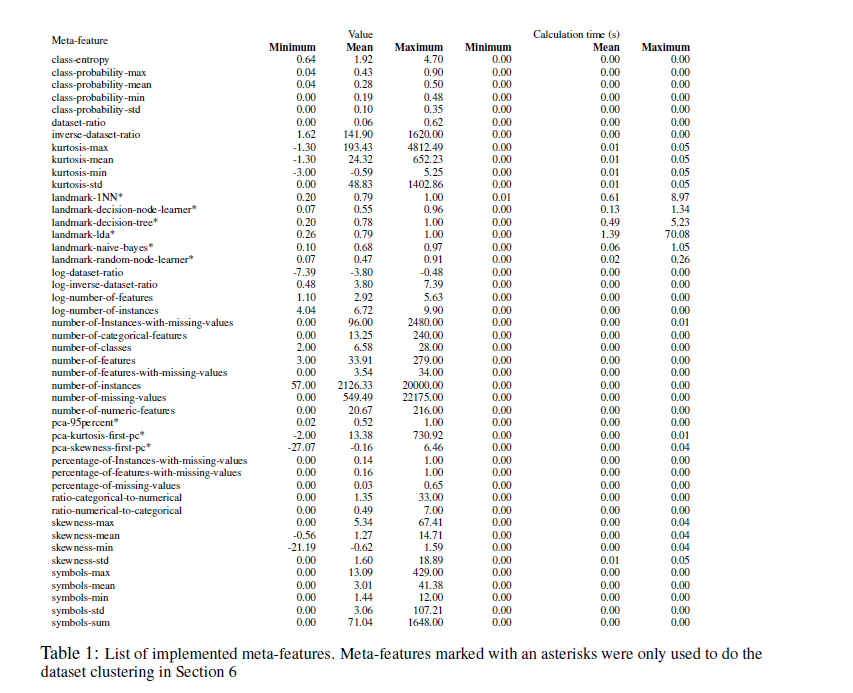
\includegraphics[width=\textwidth]{graphics/meta_features_autosklearn.png}
    \caption{Table of meta-features that were used in AUTO-SKLEARN \cite{Feurer2015EfficientLearning}.}
    \label{fig:MetaFeatureAutoSklearn}
\end{figure}
\fi

It has to be noted that the landmarking \cite{Pfahringer2000Meta-LearningAlgorithms} method was not used because of the computational complexity in the online phase, which makes it impractical in practice.

The second added component is the ensemble building component.
Instead of just taking the model that performs best, a number of models that also performed well are stored and to construct an ensemble out of them.
Because of this, the limit of just having one hyperparameter setting is lifted.
Building uniformly weighted ensemble of models found by \gls{BHO} did not work well.
Therefore ensemble selection \cite{CaruanaEnsembleModels} (which also performed better than stacking and gradient-free numerical optimization) was used.
Basically, it is a greedy procedure that starts with an empty ensemble and then iteratively adds a model that maximizes the validation performance.
\iffalse
The pseudocode is shown in \Cref{fig:ensemblePseudocode}.
\begin{figure}
\centering
    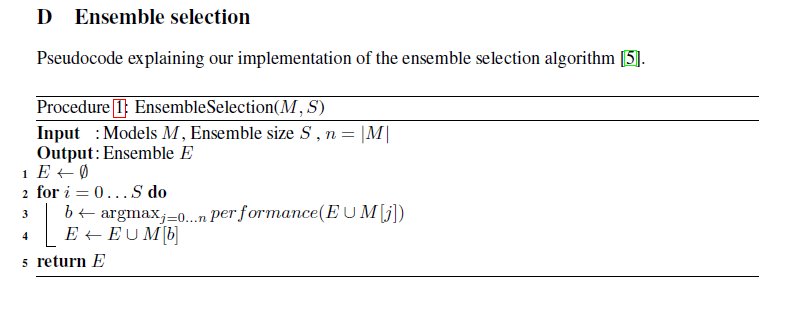
\includegraphics[width=\textwidth]{graphics/ensemble_selection_pseudocode.png}
    \caption{Pseudocode of the ensemble building algorithm \cite{Feurer2015EfficientLearning}.}
    \label{fig:ensemblePseudocode}
\end{figure}
\fi
Auto-sklearn only considered classification algorithms, so unsupervised learning methods like clustering were not taken into account.
But an important aspect of this work is to transfer the concepts of meta-learning and the used optimizers to clustering.

It has to be mentioned that there are a lot of more systems that have similar concepts, some examples are:

\begin{itemize}
    \item TPOT \cite{HomeTPOT}
    \item MLBox \cite{HomeDocumentation}
    \item H2O \cite{OverviewDocumentation}
    \item TransmogrifAI \cite{TransmogrifAIEngineering}
    \item Google Cloud AutoML \cite{CloudCloud}
    \item Microsoft Azure Automated ML \cite{AnnouncingAzure}
    \item More tools can be found in \cite{Elshawi2019AutomatedChallenges}
\end{itemize}
\xtodo{Short description for each tool? + fix reference}

\section{Meta-Learning for Clustering}

\xtodo{Overwork this. Just notes taken from the very very beginning.}

For clustering there are much less studies than for classification.

In \cite{DeSoutoRankingApproach} a meta-learning approach for ranking and selecting clustering algorithms was proposed.
They divided the architecture of their approach into three parts: \begin{inparaenum}
\item The feature extractor, which extracts the meta-features from a given dataset, 
\item the meta-learner, which applied  a regression algorithm on the extracted meta-features of the training data and applied to the validation data to generate a ranking of algorithms.
\item The database, which stores the training data with the extracted meta-features and also a ranking for this dataset for each algorithm.
\end{inparaenum}
In the first part, 8 meta-features were extracted which are mainly based on statistical
measures.
A list of this meta-features with description is given in \Cref{tab:8metafeatures}.
% Please add the following required packages to your document preamble:
% \usepackage{booktabs}
\begin{table}[]
\centering
\resizebox{\textwidth}{!}{%
\begin{tabular}{@{}ll@{}}
\toprule
Meta-feature & Description                                                                                                                                           \\ \midrule
LgE$_{10}$  & Describes the number of instances and takes it to the $log_{10}$, so LgE = $log_{10}(n)$.                                                             \\
LgREA        & Describes the log of ratio of the number of attributes by the number of instances. So LgREA = $log_{10} \frac{d}{n}$.                                 \\
PMV          & Percentage of missing data values.                                                                                                                    \\
MN           & Multivariate normality, which is the proportion of $T^2$ that are within 50 \% of the of a Chi-squared distribution.                   \\
SK           & Skewness of the $T^2$ vector.                                                                                                          \\
Chip         & Describes the type of microarray that was used (either cDNA or Affymetrix).                                                                           \\
PFA          & Percentage of attributes that were kept after the attribute selection filter.                                                                         \\
PO           & Percentage of outliers. These were measured by taking two times the $T^2$ \\
 & vector if it was two standard deviations away from the mean. \\ \bottomrule
\end{tabular}
}
\caption{List of meta-features that were used in \cite{DeSoutoRankingApproach}.}
\label{tab:8metafeatures}
\end{table}
In the second part, 7 clustering algorithms were considered: single linkage (SL), complete linkage (CL), average linkage (AL), K-means (KM), mixture model clustering (M), spectral clustering (SP) and Shared Nearest Neighbors.
The ranking was done by building a regressor for each clustering algorithm.
For this, datasets were used with the extracted meta-features.
The regression was done using the regression Support Vector Machines (rSVM) algorithm.
In the third part, the database, the dataset was stored with its meta-features and with the ranking for each algorithm. 
For each ranking, the result of an algorithm was compared to the gold-standard using the corrected Rand index \cite{Jain1988AlgorithmsData} (that index is only used for the evaluation).

The evaluation was done using 32 datasets from the micro-array domain.
They used leave-one-out crossfold for the validation, using each time 31 datasets for training and one for validation.
They assumed the ideal ranking is the ranking that was given by the corrected rand index.
Then the ranking that was generated from their meta-learner was compared to the ideal ranking by using the Spearman's rank correlation coefficient.
They showed that there approach could significantly are more correlated to the ideal ranking compared to the standard ranking.

Though they only used datasets from a very specific domain, the cancer gene expression microarray domain.
Also they did not consider the parameters at all, since they just used the "optimal" parameters.
Also they used only 8 metafeatures, where two of them can only be applied to their domain.
They also evaluated only one clustering measure, the corrected rand index, which is also an external validation measure.

In \cite{GomesFerrari2015ClusteringMethods} a similar concept for their meta-learning approach is used. 
One novelty in their approach was that they divided the set of meta-features for clustering in distance-based and attribute-based meta-features.
The distance-based meta-features were all meta-feature that can be calculated from the distance among each pair of instances in one dataset.
These include the mean, variance, standard deviation, skewness and kurtosis measures.
Also they examined how many percent of values are in a certain interval ($[0,~  0.1], ~  (0.1, ~ 0.2], \dots, ~ (0.9, ~ 1]$) and how many percent of values are in an absolute Z-score interval of $[0,~ 1),~ [1, ~ 2),~ [2, ~ 3)$ and $ [3, ~ \infty )$.
The attribute-based meta-features were meta-features that are based on the attributes of a dataset, so, e.g., the number of instances, attributes etc.
Overall 19 distance-based and 9 attribute-based meta-features were used.
They also used 7 clustering algorithms for algorithm recommendation.
For the ranking of the clustering algorithms they used different internal validation measures.
Therefore they created one ranking for each internal validation measure.
For example they used the Silhouette score and each clustering algorithm had a ranking for this measure based on the evaluated Silhouette score on the according dataset.
To combine the rankings from each of the ten internal validation measure they proposed to new methods: \begin{inparaenum}
\item The \textit{score} ranking, where each algorithm got points according to their ranking in the validation measure (e.g., 10 points for first rank, 8 for second and so on) and then the points were summed up for a new ranking.
\item The \textit{winner} ranking, where the number of victories for each validation measure was taken into account.
\end{inparaenum}
Given a new dataset, to determine which dataset is the "nearest" dataset in the meta-knowledge database, the k-Nearest-Neighbor classification algorithm was used on the meta-features.
For that purposed they also evaluated different values for the k in the kNN algorithm, ranging from 1 to 11.
There $k=5$ was used for the further experiments, because the deviation was not so high for this value.
For the evaluation also leave-one-out crossfold validation was used and to measure the performance of the recommended ranking according to the ideal ranking, Spearman's Rank Coefficient was used.
The experiments were performed on 84 datasets from the UCI repository.
They considered first only the distance-based meta-features, then the attribute-based and then hybrid based (using distance- and attribute-based meta-features) and combined all of them with every of the three ranking methods (average, score, winner).
The results showed that the best results were obtained for using the distance-based meta-features (regardlessly of the ranking method).
From the three ranking methods average, winner and score, the score ranking showed the best results.
Overall the novelty in this paper was to use the distance-based meta-features, using multiple internal indices and combine the different rankings for the algorithm by the score-ranking. 
Also they used more datasets than in the works before.
But in the evaluation the parameters for each clustering algorithm were fixed and it was not considered how to choose the best parameters or even how changing the parameters affect the results.
So they were no research done regarding hyperparameter optimization for clustering.
Also the authors state that more investigation should be done in finding more meta-features that can be extracted.

In \cite{Soares2009AnData} two meta-learners were used, the Multi-layer Perceptron (MLP) and the Support Vector Regressor (SVR).
They evaluated two sets of meta-features, which both contained 9 meta-features.
Both sets contained 4 meta-features regarding statistics about the dataset ($log_10$ of the number instances, attributes, the multivariate normality test and the percentage of outliers).
In $M_1$ the other five meta-features that contains univariate statistics (quartiles, skewness and kurtosis). 
In contrast, $M_2$ also conatains the four meta-features mentioned above and five that are based on the $T^2$ vector.
These contain three quartiles, skewness and the kurtosis of the $T^2$ vector.
For the algorithm selection, 9 clustering algorithms were taken into account and the ranking was done using a global error rate.
For the evaluation 160 arfticially generated datasets were used, which are based on an gaussian or an ellipsoid cluster generator.
The average Spearman's coefficient was used to compare the actual ranking to the ideal ranking.
The results showed that for both sets of meta-features and both meta-learners the results were more correlated to the ideal ranking than for the default ranking.

In \cite{NascimentoMiningData} meta-learning was used to derive knowledge from the training examples and to generate rules out of it, which automatically decide which clustering algorithm should be used.
For this seven clustering algorithms were used and they evaluated six meta-learning algorithms for: J48, PART, MLRules, Random Forest, k-NN and Support Vector Machine.
For the rule construction they used the MLRules algorithm and created 100 rules and selected the 10 best ones (highest weights) for the evaluation.
The evaluation was done on 36 different cancer data sets.
The extracted meta-features included the eight ones from \cite{DeSoutoRankingApproach} that can be seen in \cref{tab:8metafeatures} and extended them with 5 other meta-features. One was the normalized relative entropy (NRE), that is an indicator for the unifrom distribution of samples among classes. Then the  $SC_{10}$ and $SC_{15}$, which stand for ``small'' clusters and is a measure of number of classes with size inferior to the given thresholds 10 and 15.
They also included a similar measure for ``big'' clusters and at last the number of k-NN outliers were taken into account.

In \cite{Pimentel2019AMeta-learning} a new set of meta-features that combines correlation and dissimilarity is used, where the correlation measure is the main novelty of their approach.
In their work, 10 clustering algorithms were considered for the algorithm selection problem.
For assessing the quality of clustering results, 10 internal indices were used.
They also evaluated two meta-learners, namely the k-NN and random forests.
In the evaluation they compared their set of meta-features to other existing set of meta-features.
The experiments were performed on 219 datasets which were taken from OpenML from different domains, such as engineering, biology or physics.
Also they compared their algorithm selection system with existing ones.
The results showed that their approach performed better than the ones that are already existing in the literature when using k-NN as meta-learner.


In \cite{Corchado2019AConformations}, the authors try to estimate the number of clusters using meta-learning.
For this, they are using quality indices to describe the inner structure of the dataset.
They distinguished between two scenarios: Real-world and synthetic datasets.
The real-world datasets were categorized into binary and multi-class problems.
The aim was now to predict for a new dataset, if it is a binary or a multi-class dataset.
For the synthetic-datasets, the number of clusters ranged from 2 to 10 and in contrast to the real-world datasets, the aim was to estimate the concrete number of clusters.
The apprach was divided into three stages.
The first was the collection of meta information.´
So, how many meta-examples are used, the meta-features for each meta-example and the corresponding class label.
For the meta-features, 20 well-known inter cluster quality indices were used. 
For this, k-means was executed with for 9 different k's, ranging from $k=2$ to $k=10$, resulting in 180 meta-features that were extracted for each meta-example.
For the real-world the datasets the class label for each meta-example was either B (for binary) or MC (for multi-class).
For the synthetic datasets, the concrete number of clusters was the class label.
The second stage was the model building stage.
In this they first applied a one-class support vector machine (OCSVM) to determine if it is uniform data or not (so if they are even 2 or more clusters).
Then for those that have at least 2 or more clusters, a decision is built from the meta-features (so the qualitiy indices) using the C4.5 algorithm.
This helps to indicate which quality indices are most important (the ones on the top-level nodes and that are appearing most times).
The third stage was then the application stage, where the built model was applied to new unseen data.
For this, all 180 quality indices are computed for the new dataset and then passed to the C4.5 model, which then determined the cluster cardinality.
For the evaluation, 30 real-world datasets from the UCI repository were used, but for each of them 25 new datasets were generated using stratified sampling.
For the synthetic datasets, 2250 datasets were generated according to a cluster generator method \cite{QiuBrigham2006GenerationSeparation}.
Although the authors were able to address the problem with unsupervised data characterization predicting the number of clusters (or at least binary or not for real world datasets) using meta-learning, the effort for predicting a new unseen dataset is unacceptable high.
For a new unseen dataset, k-means has to be executed nine times (for $k=2, \cdots, 9$) and for each of this results, 20 quality indices have to be calculated. 
Also the authors did not tackle the problem of algorithm selection for clustering.

The existing literature for algorithm selection for clustering mostly use meta-learning to address this problem.
They all follow the same principle by storing meta-examples in some kind of database.
These contain meta-features together with some quality indices.
These indices are used to define an "ideal" ranking for the algorithms.
If more than one quality index is used then an aggregation of the different indices has to be defined to get one ranking for the algorithms.
When a new unseen dataset arrives, a meta-learner is used to predict the ideal algorithm for this dataset.
The most common used learners are either k-NN or random forests.
The approaches distinguish each other by different quality indices, different meta-features, different meta-learners, varying number of datasets that are used to build the meta-learning system and the number of clustering algorithms that are used.
Most of them also have in common that they do not take different parameter settings of the algorithm into account, but instead use a fixed parameter setting , which is most often the "optimal" setting if known in advance. 
The only exception here is \cite{Corchado2019AConformations} since they are trying to estimate the number of clusters using meta-learning.
But their approach is not feasible for real-world scenarios since 180 quality indices have to computed.
They also do not adress the algorithm selection problem.

\section{Hyperparameter Optimization for Clustering}

\begin{itemize}
    \item Usual process is to define search space and run clustering algorithm in this search space.
    \item Use some metric to evaluate the result.
    \item Then either choose best metric value (these are called relative metrics) or use elbow method.
    \item Also automated methods that do not require to define a search space or to run algorithm.
    \item Explain basic procedure of Xmeans \cite{Pelleg2000X-means:Clusters} /Gmeans \cite{HamerlyLearningK-means}.
    \item Basic procedure is to start with one cluster.
    \item Then split each cluster and if some criterion is met, then accept the split.
    Otherwise reject the split.
    \item Stop if no more splits were perfomred.
    \item Difference is in the criterion that can be met.
    \item Both algorithms implemented in PyClustering library \cite{NovikovPyClustering:Archive}.
    
\end{itemize}


Although the related work already investigated effort in using AutoML concepts for clustering, they still lack the following:

\begin{itemize}
    \item They did not use model-based hyperparameter optimization for clustering (like Bayesian Optimization as exmaple).
    \item There is no holistic taxonomy for the meta-features that can be used for clustering.
    \item Research was done in using algorithm selection with meta-learning or hyperparameter optimization for clustering, but it was not tried to combine both, so there is no system that considers algorithm selection and hyperparameter optimization together for clustering.
    \item Different evaluation methods were used for the ranking of the appropriate algorithms in the algorithm selection phase.
\end{itemize}

\chapter{Concept}

In this chapter the concept of transferring \gls{AutoML} concepts to clustering will be described.
For this, it will first be explained how meta-learning and the hyperparameter optimization methods were used to optimize the parameters of a clustering algorithm.
After this, the changes that had to made to the concept to also tackle the problem of algorithm selection  will be explained.


\section{Hyperparameter Optimization for Clustering}

\begin{itemize}
    \item First applied concepts on KMeans.
    \item Goal is to predict the number of clusters.
    \item For this, analyze which hyperparameter optimization methods are suitable.
    \item Also analyze which metrics are suitable for the different methods.
    \item So use internal/external metrics for the optimizers.
    \item Although external cannot be applied for new unseen datasets since they do not have class labels.
    \item But meta-learning can be used to warmstart optimizers.
    \item Warmstart means that the optimizers do not start with random models but with models that are suggestes by meta-learning model.
    \item For this, offline phase necessary.
    \item Assuming in the offline phase the number of clusters is known, it is also possible to use external metrics.
    \item Basic architecture shown in \cref{fig:concept_arch}.
    \begin{figure}
        \centering
        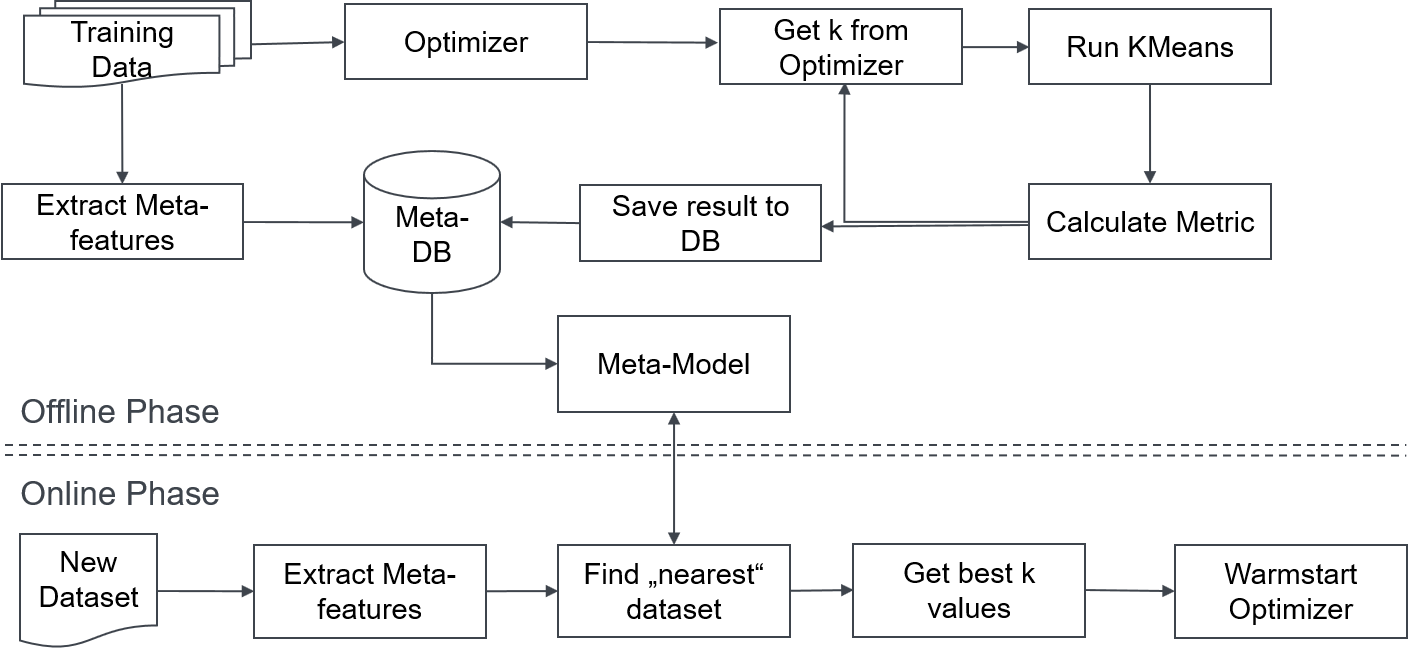
\includegraphics[width=\textwidth]{graphics/concept_architecture.png}
        \caption{General architecture of the concept divided in Online and Offline phase.}
        \label{fig:concept_arch}
    \end{figure}
    \item Offline phase: Train ``meta-model''
    \item Use optimizer to get configuration. Run KMeans on them and evaluate resulting according to metric.
    \item Then save result to Meta-DB.
    \item Also save the evaluation of the dataset together with the \textit{meta-features}.
    \item Meta-DB builds the meta-model.
    \item For the meta-model a k-NN classifier with $k=1$ is used.
    \item If new dataset has to be clustered in online phase, then extract meta-features (same as in offline phase). 
    \item Then find the ``nearest'' dataset.
    This is basically where 1-NN is used to find the nearest dataset based on the $L1$ distance.
    \item Input is meta-features of the new dataset and these are used to build the 1-NN and find the nearest dataset.
    \item From the nearest dataset it is looked up for which configurations the lowest k deviation was measured in the offline phase.
    \item This configurations are then used to \textit{warmstart} the optimizer, which means the optimizer first evaluates this configurations.
    
    
    
    
\end{itemize}
 
 
\section{Algorithm Selection for Clustering}

\begin{itemize}
    \item Basically same as for Hyperparameter Selection.
    \item Instead of only using parameters of that one algorithm, the optimizer gets one additional parameter.
    \item Additional parameter is name of algorithm.
    \item So the optimizer predicts the name of the algorithm and the hyperparameters like done in \cite{ThorntonAuto-WEKA:Algorithms}.
    \item Limited to partitional clustering algorithms.
    \item Basically Bayes would also be applicable to other clustering algorithms, but for multi-arm bandit based methods the budget has to be defined somehow.
    To get a meaningful metric result one needs labels for all data points after each iteration if the budget is the number of iterations or even for time budget.
    This holds partitional clustering algorithms but not necessarily for other kinds of clustering algorithms.
    \item The architecture shown in \cref{fig:concept_arch} changes in that way that the optimizer does not only gives the k value that should be executed next, but also the algorithm.
    \item New architecture can be seen in \cref{fig:archAlgoSelection}.
    \begin{figure}
        \centering
        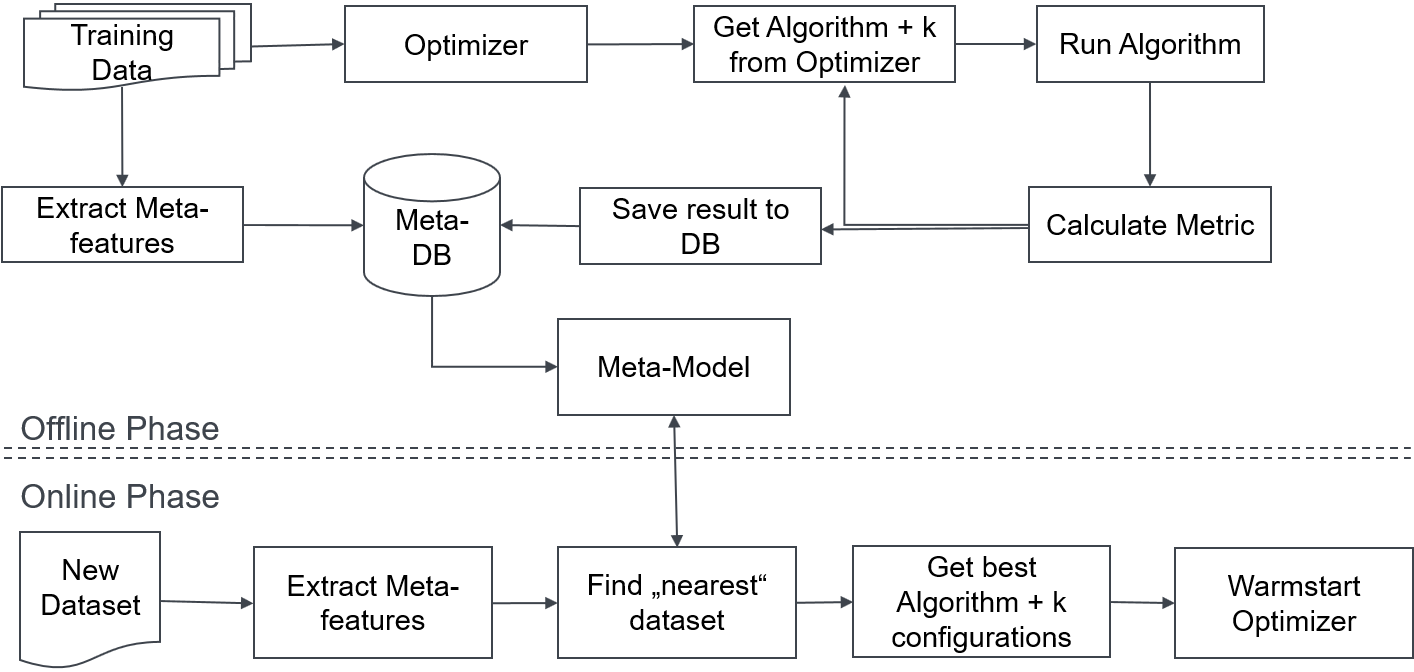
\includegraphics[width=\textwidth]{main/concept_architecture_algo_selection.png}
        \caption{General architecture of the concept to also include the algorithm selection.}
        \label{fig:archAlgoSelection}
    \end{figure}
    
\end{itemize}

\chapter{Implementation}

In this chapter the implementation details will be described.
For this, first the used technologies are explained.
After this, the database schema that was used for storing the meta-features and the evaluations will be described.
Last but not least the used algorithms, optimizers and features will be mentioned.

\section{Technologies}

\begin{itemize}
    \item Python as programming language
    \item scikit-learn \cite{PedregosaFABIANPEDREGOSA2011Scikit-learn:Perrot} as library for implementing the algorithms and the metrics.
    \item Used algorithms KMeans, KMedoids\cite{Kaufman1987ClusteringMedoids} and GMM. 
    Implementations taken from scikit-learn, besides KMedoids which was taken from scikit-learn extra\footnote{https://scikit-learn-extra.readthedocs.io/en/latest/user_guide.html#k-medoids}.
    \item For all algorithms the number of max iterations were set to 10.
    \item KMeans was implemented using the  \textit{k-means++} \cite{Arthur2007K-means++:Seeding} method
    and KMedoids with a similar method, called \textit{k-medoids++}.
    \item The metrics that were used were all that are implemented in scikit-learn, which means 6 external and 3 internal were used.
    \item The Silhouette coefficient \cite{Rousseeuw1987Silhouettes:Analysis} was implemented using only 10\% of the data with random sampling.
    \item The reason is the high runtime which would exceed the possibilities and resources of this work.
    \item For the online phase only the 3 internal metrics were used. 
    \item The optimizers that were used were all that were described in ... \xtodo{reference here background section of optimizers}
    \item The implementation of the Random and the Bayes optimizer was done using the scikit-optimize \cite{Head2018Scikit-optimize} implementation.
    \item Reason for this library: in python, easy to add warmstarting, ask-and-tell interface.
    \item The Hyperband and BOHB optimizers were implemented using the implementation mentioned in \cite{Falkner2018BOHB:Scale}, which contains an implementation for both Hyperband and BOHB.
    \item The architecture was kept quite flexible so that running each optimizer which each metric on each implemented algorithm is possible.
    \item Goal is to compare the different optimizers and metrics per optimizer.
    \item Relational database was used because the relationship between the metafeatures, dataset and the results of the optimizers need to be stored.
    \item Also the schema should not change.
    \item PostgreSQL\footnote{https://www.postgresql.org/} used as database.
    \item The meta-feature extraction was done using the pymfe\footnote{https://pypi.org/project/pymfe/} \cite{Rivolli2018TowardsMeta-learning} package.
    \item For this all meta-features were used that do not need class labels.
\end{itemize}

\section{Database Schema}
\begin{itemize}
    \item For accessing the PostgreSQL database instance, the python package SQLAlchemy \cite{sqlalchemy} was used.
    \item More specific, the Object-relational mapper was used.
    \item Schema of the database is shown in \cref{fig:dbschema}.
    Describe in more detail.
    \begin{figure}
        \centering
        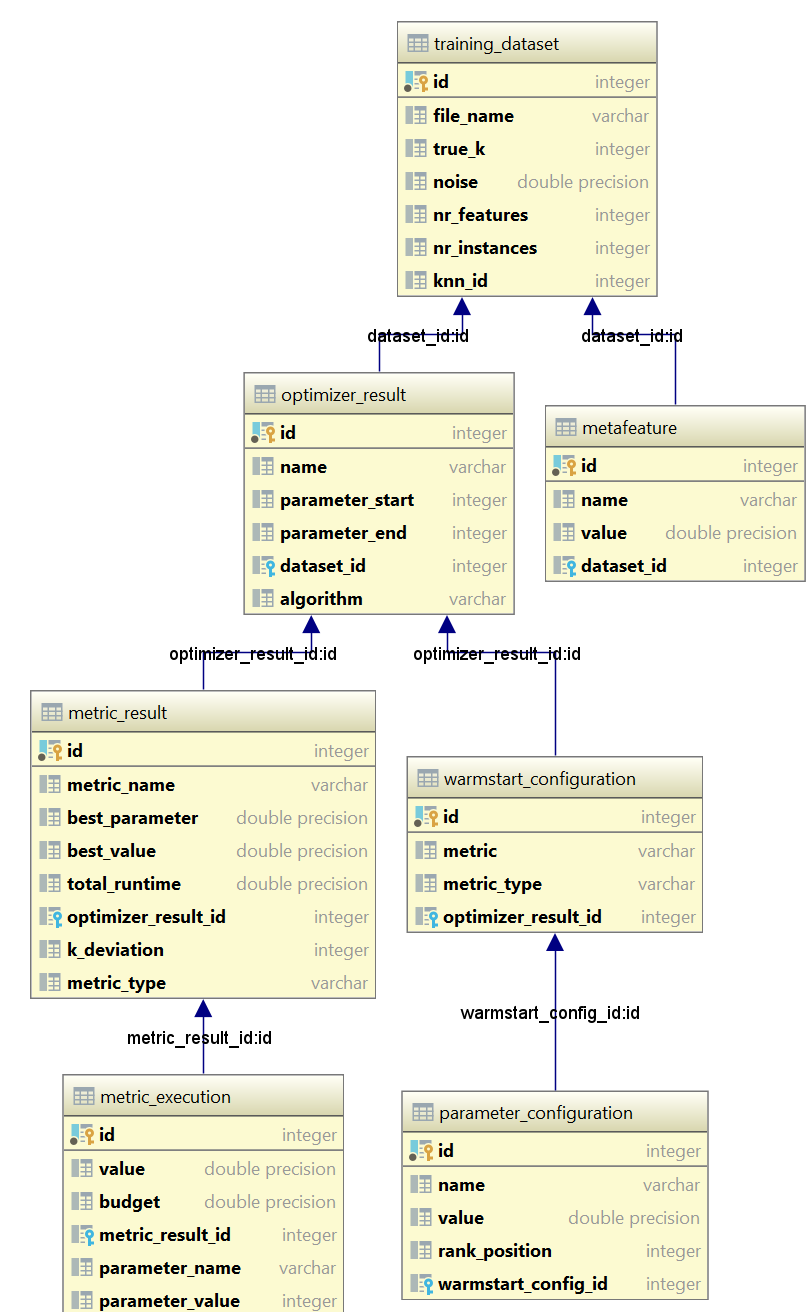
\includegraphics[width=0.7\textwidth]{graphics/database_schema.png}
        \caption{Overview of the database schema that was used to store the meta-features as well as the results of the optimizers.}
        \label{fig:dbschema}
    \end{figure}
    
    \xtodo{Show schema for algo selection as well and explain difference? But actually not that much changed...}
\end{itemize}

\section{Generation of Training and Test Datasets}

In this section the datasets that were used for the evaluation will be described.
\begin{itemize}
    \item For Offline phase of the concept, training data is needed.
    \item Introduce notation
    \item 
\end{itemize}




\chapter{Evaluation of Hyperparameter Selection}

\section{Offline}

\subsection{Setup}

\begin{itemize}
    \item For the evaluation, 81 datasets that were all synthetically generated were used.
    \item For the generation of the dataset the tool described in \cite{Fritz2019InitializingAnalysis} was used. \xtodo{Maybe move this part to implementation? And then only describe the used input parameters. Or maybe describe also training and test data generation with used parameters in implementation}
    \item The generated the datasets based on the following input parameters:
    \begin{itemize}
        \item $n$: Number of instances of the dataset.
        \item $d$: Number of dimensions (or features) of the dataset.
        The value of each generated feature was in the intervall [-10, 10].
        \item $k$: Number of clusters of the dataset. Each cluster was generated according to the Gaussian distribution with mean at the center and standard deviation of 0.5.
        Also, each cluster contained $\frac{n}{k}$ instances.
        \item $r$: Ratio of outliers of the dataset. This means that $\frac{r}{100} \ast n$ additional instances were added uniformly.
    \end{itemize}
    \item Each of the input parameters was divided into three categories: \textit{Small}, \textit{Medium} and \textit{Large}.
    \item The values for each category and input parameter for the offline phase can bee seen in \cref{tab:parametersOfflinePhase}.
    
% Please add the following required packages to your document preamble:
% \usepackage{booktabs}
\begin{table}[]
\centering
\caption{The values of the input parameters for the generation of the training datasets divided into \textit{Small}, \textit{Medium} and \textit{Large}.}
\label{tab:parametersOfflinePhase}
\begin{tabular}{@{}llll@{}}
\toprule
Parameter    & Small & Medium & Large  \\ \midrule
$n$ & 1,000 & 5,000  & 10,000 \\
$d$ & 10    & 30     & 50     \\
$k$ & 5     & 50     & 100    \\
$r$ & 0     & 33     & 66     \\ \bottomrule
\end{tabular}
\end{table}
\item For each combination of parameters one dataset was created.
\item Since there are $3^4 = 81$ combinations, the same amount of datasets was created for the training phase.
\item Because 9 metrics, 4 optimizers and 81 datasets were used, 2,916 optimizer runs were performed.
\item Each optimizer had 50 iterations, which results in 145,800 KMeans and metric executions.
\item Therefore, the range for the possible $k$ values that were sampled from the optimizers were limited to $R=[2, 2 * k_{max}]$, where $k_{max}$ denotes the highest actual k value that was used in the generated datasets.
Since $k_{max}=100$ the range was set to $R=[2, 200]$.
\item Theoretically, the range could be $[2, n]$ but this would be computational too expensive.
\item A value close to $n$ would mean that the runtime complexity of KMeans would be quadratic.
\item 
\end{itemize}
\section{Online}



% Please add the following required packages to your document preamble:
% \usepackage{booktabs}
\begin{table}[]
\centering
\caption{The values of the input parameters for the generation of the training datasets divided into \textbackslash{}textit\{Small\}, \textbackslash{}textit\{Medium\} and \textbackslash{}textit\{Large\}.}
\label{tab:parametersOfflinePhase}
\begin{tabular}{@{}lllll@{}}
\toprule
       & $n$    & $d$ & $k$ & $r$ \\ \midrule
Small  & 1,000  & 10  & 5   & 0   \\
Medium & 5,000  & 30  & 50  & 33  \\
Large  & 10,000 & 50  & 100 & 66  \\ \bottomrule
\end{tabular}
\end{table}
\subsection{Coldstart}

\subsection{Warmstart}

\chapter{Evaluation of Combined Algorithm and Hyperparameter Selection}

\section{Offline}

\section{Online}

\subsection{Coldstart}

\subsection{Warmstart}

\chapter{Conclusion}
\label{chap:zusfas}

\section*{Outlook}
\cite{Weiss2016ALearning}
\printbibliography

All links were last followed on March 17, 2019.

\appendix

\pagestyle{empty}
\renewcommand*{\chapterpagestyle}{empty}
\Versicherung
\end{document}
